\PassOptionsToPackage{table}{xcolor}

\documentclass[sigconf%
,natbib=true%
]{acmart}

\AtBeginDocument{%
  \providecommand\BibTeX{{%
    \normalfont B\kern-0.5em{\scshape i\kern-0.25em b}\kern-0.8em\TeX}}}

\copyrightyear{2021} 
\acmYear{2021} 
\setcopyright{rightsretained} 
\acmConference[VINCI '21]{The 14th International Symposium on Visual Information Communication and Interaction}{September 6--8, 2021}{Potsdam, Germany}
\acmBooktitle{The 14th International Symposium on Visual Information Communication and Interaction (VINCI '21), September 6--8, 2021, Potsdam, Germany}\acmDOI{10.1145/3481549.3481570}
\acmISBN{978-1-4503-8647-0/21/09}

\usepackage[utf8]{inputenc}
\usepackage{csquotes}
\usepackage{tabto}
\usepackage{enumitem}
\usepackage{calc}
\usepackage[ruled,vlined,linesnumbered]{algorithm2e}
\SetAlFnt{\small}
\SetAlCapFnt{\footnotesize}
\SetAlCapNameFnt{\footnotesize}
\usepackage{tabularx}
\usepackage{multirow}
\usepackage{hhline}
\usepackage{makecell}

\usepackage{pifont}

\usepackage{tikz}
\usepackage{eso-pic}
\AddToShipoutPictureFG{\AtPageLowerLeft{\put(\LenToUnit{0.5\paperwidth},\LenToUnit{6mm}){\makebox[0pt][c]{\fontsize{6.5}{8}\selectfont\color{gray}Author's revised version (2026-11-08). Version of record: \url{https://doi.org/10.1145/3481549.3481570}}}}}
\usetikzlibrary{calc,positioning,spy}

\newcommand*\rot{\rotatebox{90}}
\newcommand*\rotc{\rotatebox[origin=rb]{270}}
\newcommand*\OK{$\bullet$}
\newcommand*\UP{\ding{218}}
\newcommand*\DOWN{\ding{216}}
\newcommand*\rhombusOK{\ding{70}}
\newcommand*\significOK{$\star$}
\newcommand*\notsignificOK{$\diamond$}

\newcommand*\PARTIAL{$\circ$}
\newcommand*\NA{\cellcolor{gray!40}}
\newcommand*\UNKNOWN{--}

% KwInMulti and KwOutMulti commands
\newlength\mylenin
\newcommand\KwInMulti[1]{%
  \settowidth\mylenin{\KwIn{}}%
  \setlength\hangindent{\mylenin}%
  \hspace*{\mylenin}#1\\}
  
\newlength\mylenout
\newcommand\KwOutMulti[1]{%
  \settowidth\mylenout{\KwOut{}}%
  \setlength\hangindent{\mylenout}%
  \hspace*{\mylenout}#1\\}

% FuncName command
\newcommand{\FuncName}[1]{\mbox{\normalfont\textsc{#1}}}

\begin{document}

\title[Visualization of Data Changes in 2.5D Treemaps using Procedural Textures and Animated Transitions]{Visualization of Data Changes in 2.5D Treemaps using\\Procedural Textures and Animated Transitions}

\author{Daniel Limberger}
\orcid{0000-0002-9111-4809}
\affiliation{%
  \institution{Hasso Plattner Institute, Digital Engineering Faculty,}
  \country{University of Potsdam, Germany}
}
\author{Willy Scheibel}
\orcid{0000-0002-7885-9857}
\affiliation{%
  \institution{Hasso Plattner Institute, Digital Engineering Faculty,}
  \country{University of Potsdam, Germany}
}
\author{Jan van Dieken}
\affiliation{%
  \institution{Hasso Plattner Institute, Digital Engineering Faculty,}
  \country{University of Potsdam, Germany}
}
\author{J{\"u}rgen D{\"o}llner}
\affiliation{%
  \institution{Hasso Plattner Institute, Digital Engineering Faculty,}
  \country{University of Potsdam, Germany}
}

\renewcommand{\shortauthors}{D.~Limberger, W.~Scheibel, J.~v.~Dieken, J.~D{\"o}llner}

\begin{abstract}
    This work investigates the extent to which animated procedural texture patterns can be used to support the representation of changes in 2.5D treemaps.
    Changes in height, color, and area of individual nodes can easily be visualized using animated transitions.
    Especially for changes in the color attribute, plain animated transitions are not able to directly communicate the direction of change itself.
    We show how procedural texture patterns can be superimposed onto the color mapping and support transitions.
    To this end, we discuss qualitative properties of each pattern, demonstrate their ability to communicate change direction both with and without animation, and conclude which of the patterns are more likely to increase effectiveness and correctness of the change mapping in 2.5D treemaps.
\end{abstract}

\begin{CCSXML}
	<ccs2012>
	<concept>
	<concept_id>10003120.10003145.10003146.10010889</concept_id>
	<concept_desc>Human-centered computing~Treemaps</concept_desc>
	<concept_significance>500</concept_significance>
	</concept>
	<concept>
	<concept_id>10003120.10003145.10003147.10010923</concept_id>
	<concept_desc>Human-centered computing~Information visualization</concept_desc>
	<concept_significance>300</concept_significance>
	</concept>
	</ccs2012>
\end{CCSXML}

\ccsdesc[500]{Human-centered computing~Treemaps}
\ccsdesc[300]{Human-centered computing~Information visualization}

\keywords{visualization, time-variant data, change visualization, 2.5D treemaps, animated transitions, procedural textures, read direction}

\maketitle
\hypersetup{pdftitle={Visualization of Data Changes in 2.5D Treemaps using Procedural Textures and Animated Transitions}}

\section{Introduction}
\begin{figure}[t]
    \begin{tikzpicture}[spy using outlines={white, rectangle, magnification=2.5, size=64, connect spies, every spy on node/.append style={line width=1.0pt}},inner sep=0pt, outer sep=0pt]
        \node[anchor=west](arrows0) at (0,0) {%
            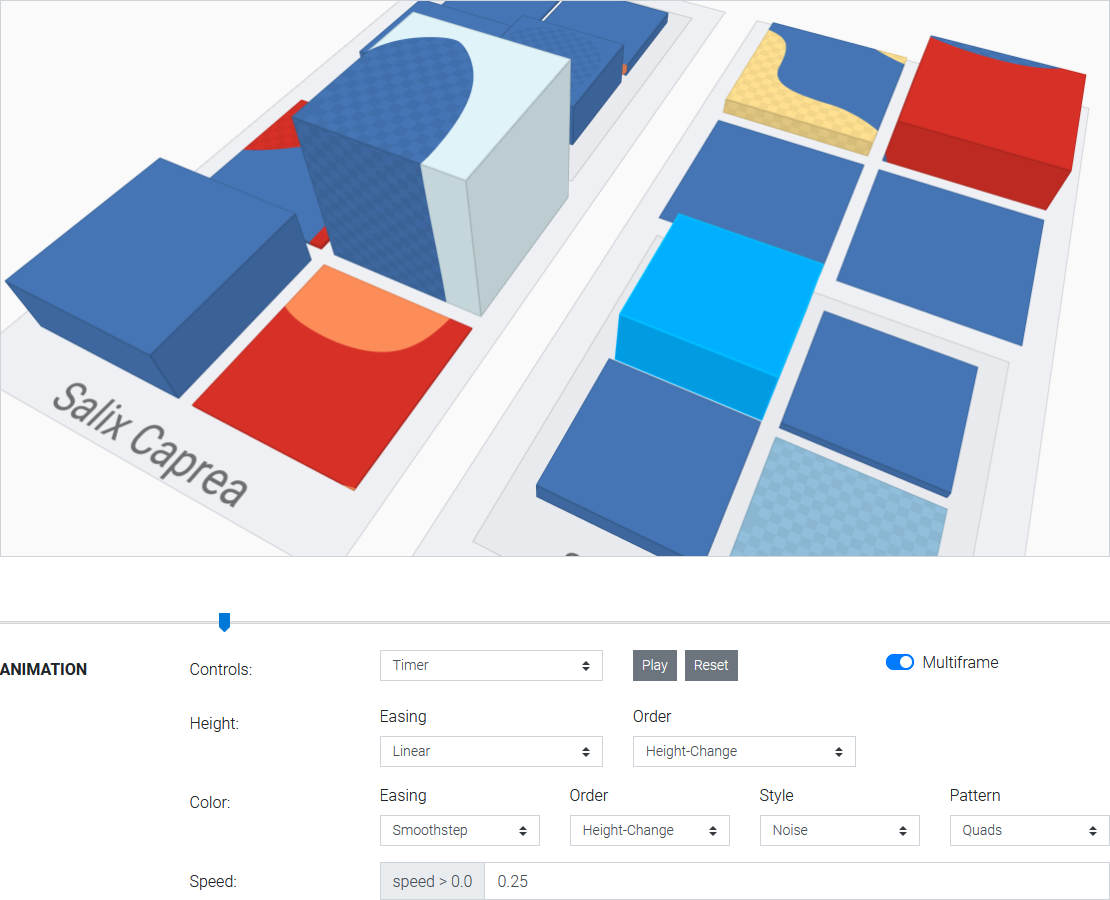
\includegraphics[width=1.0\linewidth, trim=0 48 0 0, clip]{figures/teaser}};
        \spy [white] on ($(arrows0.center)+(-1.0, +2.25)$) in node at ($(+2.0, +1.0)+(arrows0.center)$);
    \end{tikzpicture}
    \caption{Tiny hierarchical test data set depicted using a 2.5D treemap that allows transitioning between subsequent values in time-series data mapped to area, height, and color. A combination of two of our procedural patterns is used to animate changes in subsequent values mapped to color.}
    \label{fig:teaser}
\end{figure}
Treemaps have become a highly expressive tool for visualizing hierarchical, multi-variate data in a variety of domains, including software data~\cite{limberger2019-softwaremaps}.
Typically, the data represented has a timestamp and changes over time.
Software maps, for example, can represent aspects of a software system for a specific revision or time.
We want to enable users to interactively explore correlations in time-varying software system engineering data, i.e., metrics per revision, development budgets, status and progress of defects and issues, team composition, development activity, etc.
An explicit mapping of the difference between two subsequent states to color or height would be the first choice.
For 2D treemaps, color patterns such as \emph{two corners}---resulting in a diagonal color gradient---or contrast modifications like \emph{ratio shading} can be used~\cite{tu2007-changes}.
The time dimension can further be incorporated by distributing multiple maps spatially using small multiples~\cite{scheibel2016-smallmultiples,chen2017-pesticide}.
Provided the evolution (over more than just two states) is already analyzed and available by means of trend data, natural metaphors such as physically based material degradation, shininess, or glyphs can be an effective tool for communication~\cite{wurfel2016-naturalphenomena}.

We want to assist height and color mappings already in use (\emph{map themes}) and intrinsically emphasize temporal changes, but rely on the user's existing understanding of treemaps.
Thereby, the representation of change should visually correspond to the change in data (\emph{visual-data-correspondence})~\cite{kindlmann2014-algebraic}, i.e., the actual difference between two values and the direction of change (or sign of the difference).
For this, basic variants of \emph{data vases}~\cite{thakur2009-datavases}, glyphs~\cite{pires2020-glyphs}, or \emph{in-situ templates}~\cite{limberger2019-insitu} can be used.
The latter allow for change encoding of up to three visual variables simultaneously, though, ample training is required and issues with reading direction must be considered.
A simple but effective use of in-situ templates for display of changes in height is given in~\autoref{fig:static-display}, one using explicit color mapping (thereby partially occluding the actual color mapping) the other a procedural pattern for direction encoding (using an arrow pattern).
Alternatively, animation by means of an interpolation of height and color attributes~\cite{bladh2005-transitions,langelier2008-evolution} could be used. 

In this work, we combine these two approaches: we utilize procedural texture patterns for more effective animated transitions~(\autoref{fig:teaser}).
Our main contributions are
\begin{itemize}
    \item the introduction of procedural texture patterns that are suitable for mapping change in color in 2.5D treemaps,
    \item the idea of primary and secondary patterns for accurate display of change direction when the animation is paused,
    \item the evaluation of said patterns w.r.t. their applicability under various constraints and circumstances.
\end{itemize}

\begin{figure}[t]
    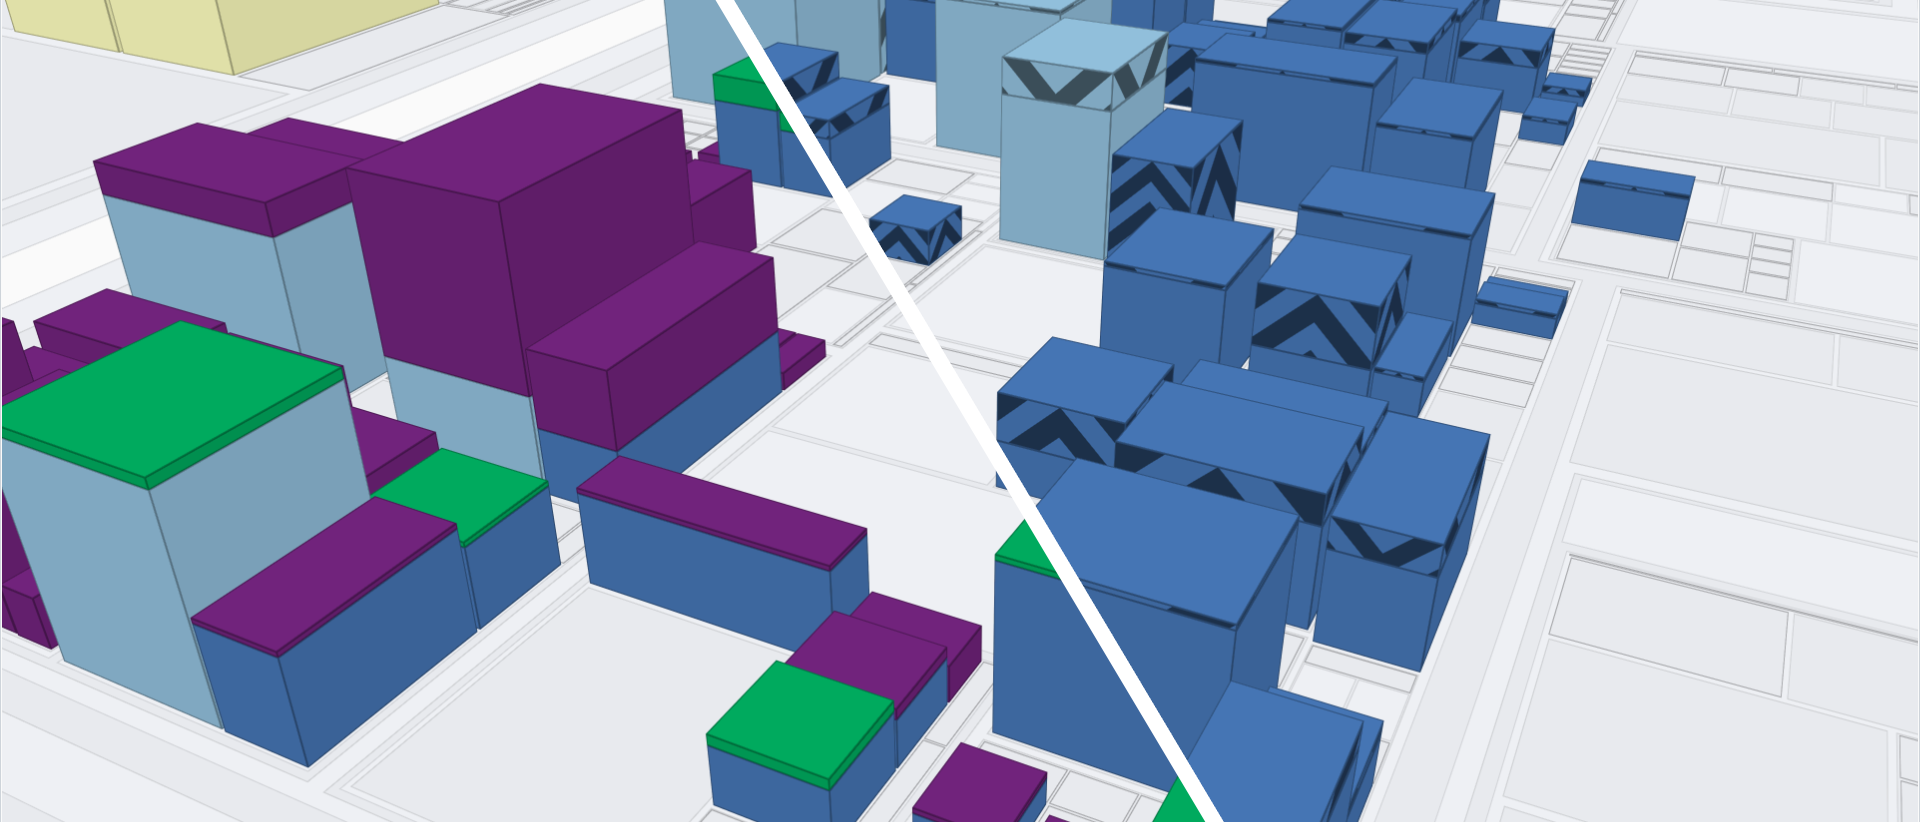
\includegraphics[width=\linewidth]{figures/treemap-static-classic-219}
    \caption{Basic approach for communicating the delta between subsequent values mapped to height: colors (left) and arrows (right) mapped to the delta in height.}
    \label{fig:static-display}
\end{figure}

\section{Patterns for Animated Transitions}
We propose seven patterns that can encode the transition between two colors.
As these patterns share approaches but also differ in their visual display and characteristics to encode additional state or ensure certain invariants regarding the encoding, we introduce the alternatives and compare them (\autoref{sec:evaluation}).

\subsection{Procedural Texture Patterns}
A pattern describes a mapping of a transition progress for a fragment on a cuboid's surface resulting in a binary per-fragment choice of color.
This is done using \emph{signed-distance-functions}~\cite{Vivo} and fragment shaders.
The patterns differ mainly in their appearance, granularity, and the surfaces they are intended for.
\begin{figure}[tbp]
    \begin{tikzpicture}[spy using outlines={white, rectangle, magnification=2.5, size=32, connect spies, every spy on node/.append style={line width=1.0pt}},inner sep=0pt, outer sep=0pt]
        \node[anchor=west](arrows0) at (0,0) {%
            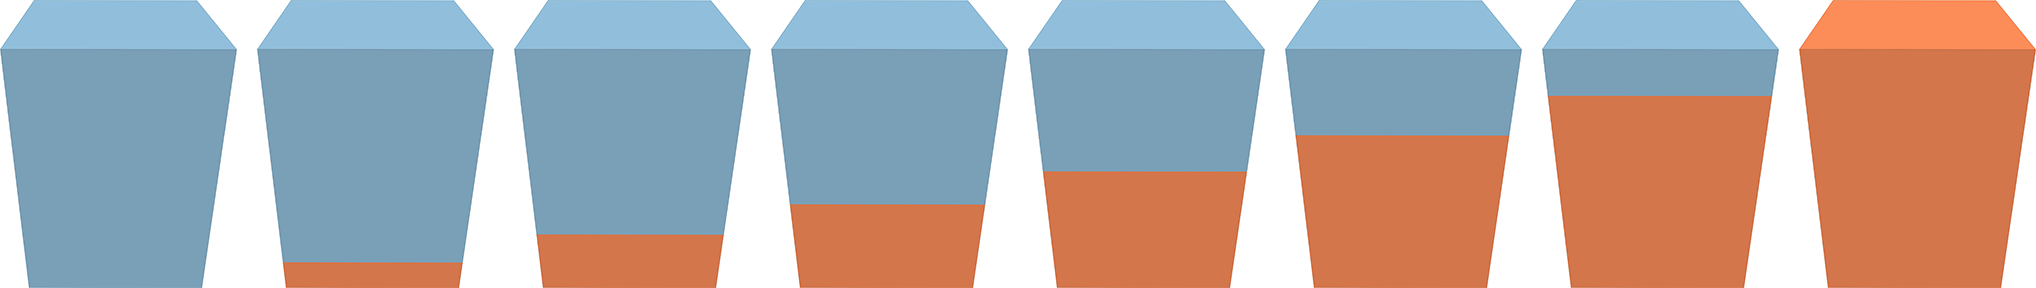
\includegraphics[width=1.0\linewidth]{figures/basic-trans-vars-vertical}};
        \node[below=1.5cm of arrows0.south,anchor=west](arrows1) at (0,0) {%
           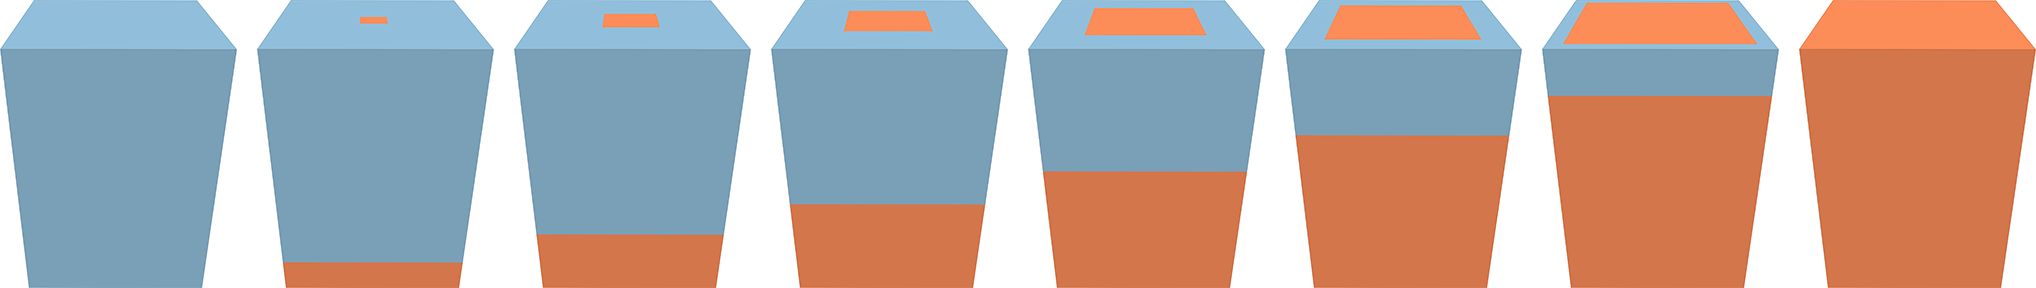
\includegraphics[width=1.0\linewidth]{figures/basic-trans-vars-pyramid}};%
        \node[below=3.0cm of arrows1.south,anchor=west](arrows2) at (0,0) {%
           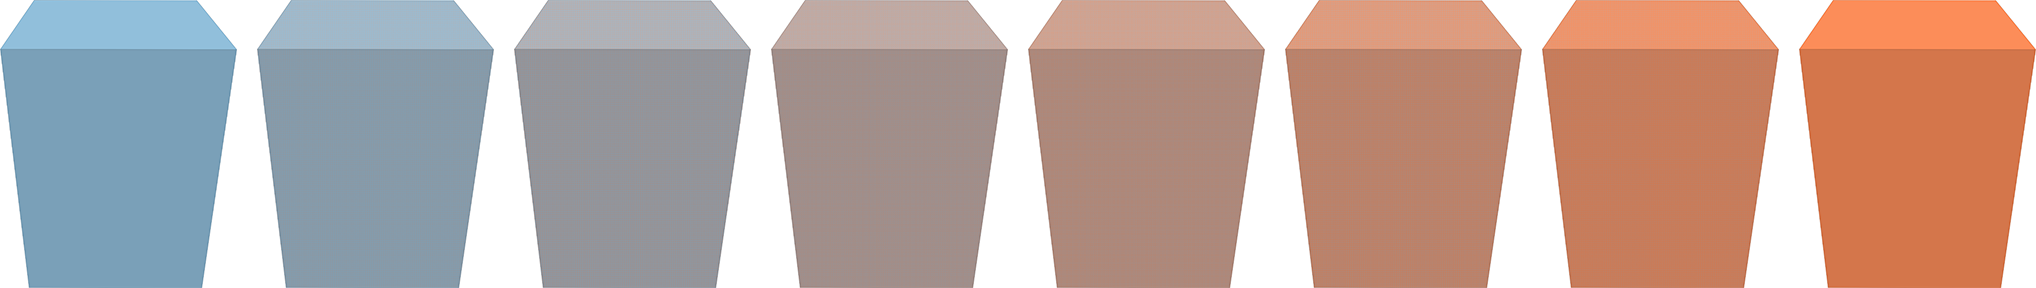
\includegraphics[width=1.0\linewidth]{figures/basic-trans-vars-dithering}};%
        \node[below=4.5cm of arrows2.south,anchor=west](arrows3) at (0,0) {%
           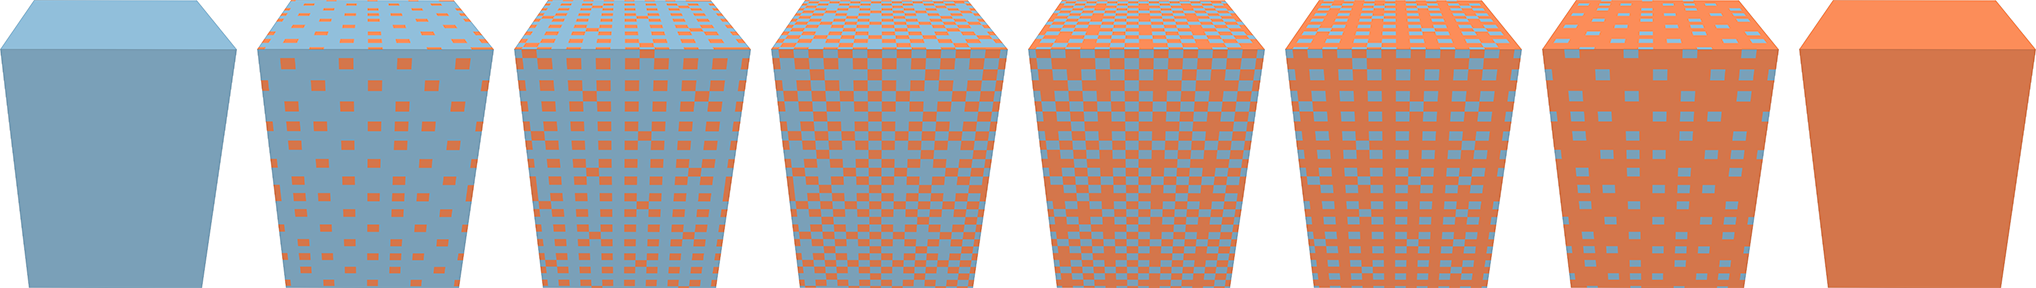
\includegraphics[width=1.0\linewidth]{figures/basic-trans-vars-quads}};%
        \node[below=6.0cm of arrows3.south,anchor=west](arrows4) at (0,0) {%
           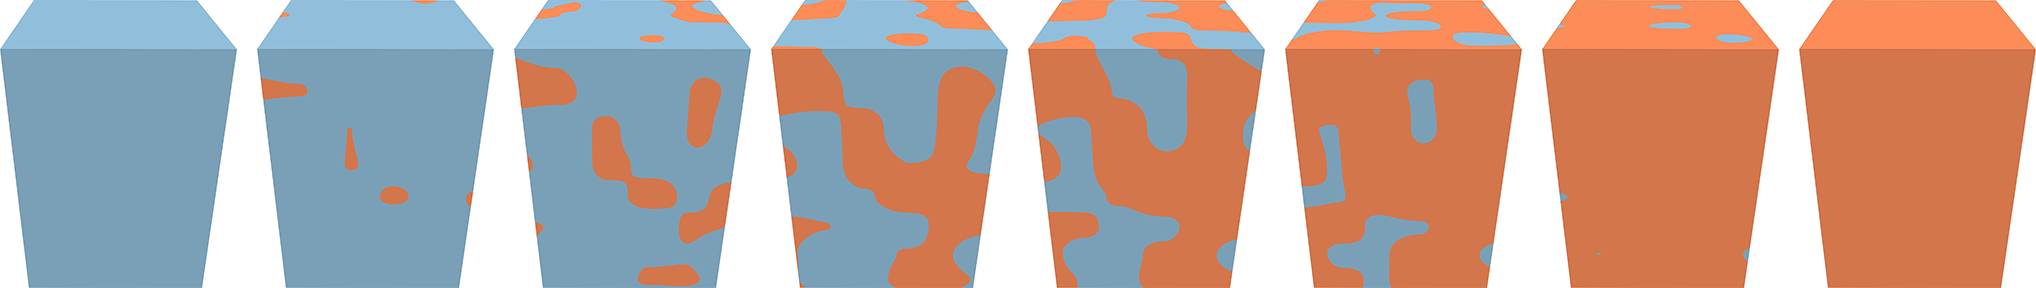
\includegraphics[width=1.0\linewidth]{figures/basic-trans-vars-noise}};%
        \spy [white] on ($(arrows2.center)+(+0.45, +0.325)$) in node at ($(+2.0, +0.25)+(arrows2.center)$);
        \spy [white] on ($(arrows3.center)+(+0.45, +0.325)$) in node at ($(+2.0, +0.25)+(arrows3.center)$);
        \spy [white] on ($(arrows4.center)+(+0.45, +0.325)$) in node at ($(+2.0, +0.25)+(arrows4.center)$);
    \end{tikzpicture}
    \caption{Procedural patterns for changes in color attribute, from top to bottom: pillar, pyramid, dithering, squares, and noise. All of the above are not capable of encoding the direction of change ($\Delta_{\textrm{DirChange}}$) when animation is paused.}
    \label{fig:basic-trans-vars}
\end{figure}

\paragraph{Pillar (vertical)}
The pillar pattern dissects the surface vertically and assigns the former color and next color to a top share and a bottom share of the pillar, respectively (\autoref{fig:basic-trans-vars}).
A transition using this pattern starts with a full pillar using the former color.
Then, the next color \emph{grows} from the top and overlays the former color step by step.
Thus, after a brief training period, a user should be able to determine the former color and the next color, even for a static display.
However, this pattern does not show partial progress on the top faces.
Instead, the color of the top face changes instantaneously with the completion of the transition.

\paragraph{Pyramid (vertical)}
The pyramid pattern is an extension to the pillar pattern w.r.t. explicit handling of the top faces.
The lateral faces use the same encoding.
However, the pattern name \emph{pyramid} describes the metaphorical process that is used to derive the pattern: a virtual pyramid is embedded in the cuboid and slowly pushed towards and through the top of it (\autoref{fig:basic-trans-vars}).
All cuboid fragments that intersect with the pyramid are assigned the upcoming color.
This intersection surface corresponds to the progress of the pillar template for lateral faces and results in a growing rectangle for top faces.
As a result, this pattern encodes the current progress of transition on both the lateral faces and the top face.

\paragraph{Noise}
The noise pattern uses a 3D noise function~\cite{Perlin01} and a threshold to discriminate the surface for the two colors.
Using such a pattern results in organic-looking surfaces and transition behavior (\autoref{fig:basic-trans-vars}).
However, a sensible parameterization of the noise w.r.t. the scaling is challenging.
As one approach we propose to approximate the scale factor by the number of nodes in the tree.

\paragraph{Dithering}
The dithering pattern encodes the transition using a per-pixel dithering pattern (\autoref{fig:basic-trans-vars}).
The dithering is applied in screen space and from a perceptional point of view, this results in a visual blending of the two colors \cite{Ulichney88}.
However, using dithering we assert that only actual colors from a color scheme will be used.

\paragraph{Squares}
The squares pattern extends the dithering by using areas larger than one pixel for the dithering raster (\autoref{fig:basic-trans-vars}).
As another difference, the pattern is applied in the world space of the treemap and not the raster on the screen.
This reduces the visual blurring of colors while providing a transition nonetheless.
\begin{figure}[tbp]
    \begin{tikzpicture}[spy using outlines={white, rectangle, magnification=2.5, size=32, connect spies, every spy on node/.append style={line width=1.0pt}},inner sep=0pt, outer sep=0pt]
        \node[anchor=west](arrows0) at (0,0) {%
            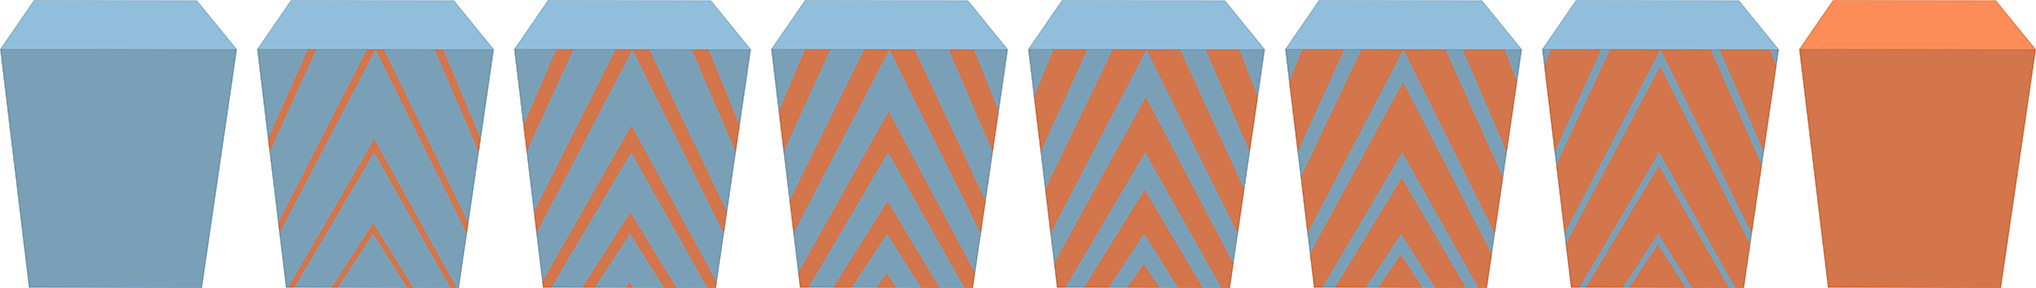
\includegraphics[width=1.0\linewidth]{figures/arrow-trans-vars}};
        \node[below=1.5cm of arrows0.south,anchor=west](arrows1) at (0,0) {%
           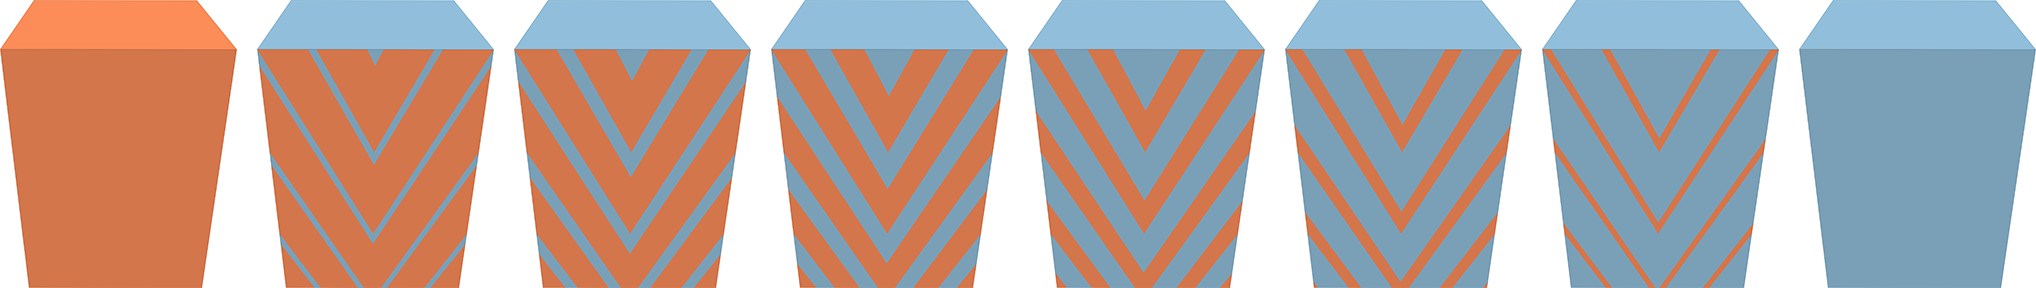
\includegraphics[width=1.0\linewidth]{figures/arrow-trans-vars-inverse}};%
        \spy [white] on ($(arrows0.center)+(+0.45, +0.325)$) in node at ($(+2.0, +0.25)+(arrows0.center)$);
        \spy [white] on ($(arrows1.center)+(+0.45, +0.325)$) in node at ($(+2.0, +0.25)+(arrows1.center)$);
    \end{tikzpicture}
    \caption{Arrow pattern filling up the color display for increasing (top) or decreasing (bottom) values. The arrows encode value increase or decrease resp., even when paused.}
    \label{fig:arrow-trans-vars}
\end{figure}

\paragraph{Arrows} % (lateral)
This pattern is a modulated, two-dim\-en\-sion\-al \emph{abs} function applied to every lateral face individually.
The top faces behave similarly to the pillar pattern.
In contrast to the pillar and pyramid patterns, the arrow direction can encode the direction of value change, as the arrows can point upwards or downwards~(\autoref{fig:arrow-trans-vars}).
This, however, prevents effective encoding of direction of animation.
\begin{figure}[tbp]
    \begin{tikzpicture}[spy using outlines={white, rectangle, magnification=2.5, size=32, connect spies, every spy on node/.append style={line width=1.0pt}},inner sep=0pt, outer sep=0pt]
        \node[anchor=west](arrows0) at (0,0) {%
            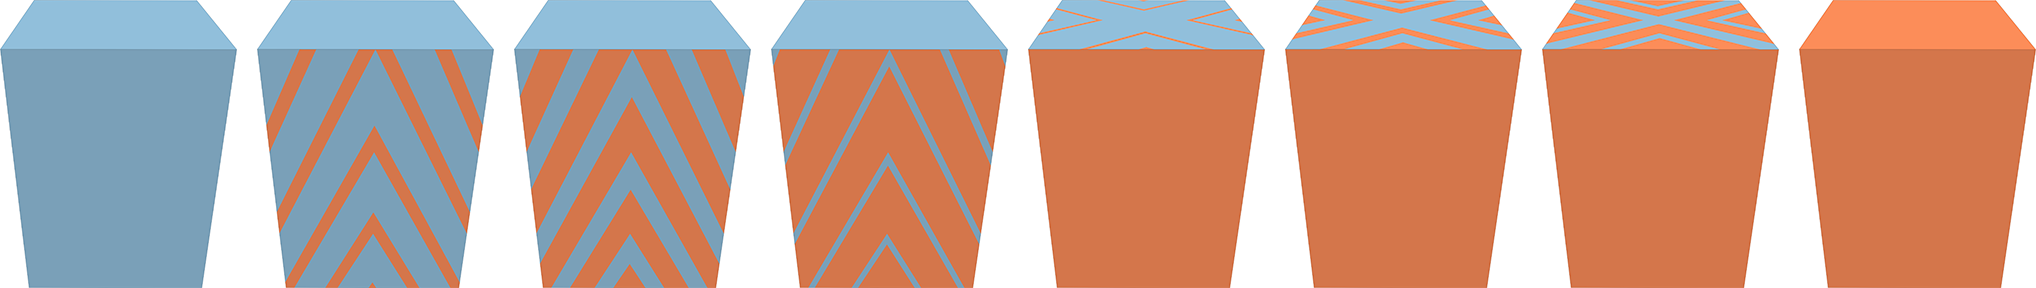
\includegraphics[width=1.0\linewidth]{figures/arrow-trans-vars-variants-divided}};
        \node[below=1.5cm of arrows0.south,anchor=west](arrows1) at (0,0) {%
           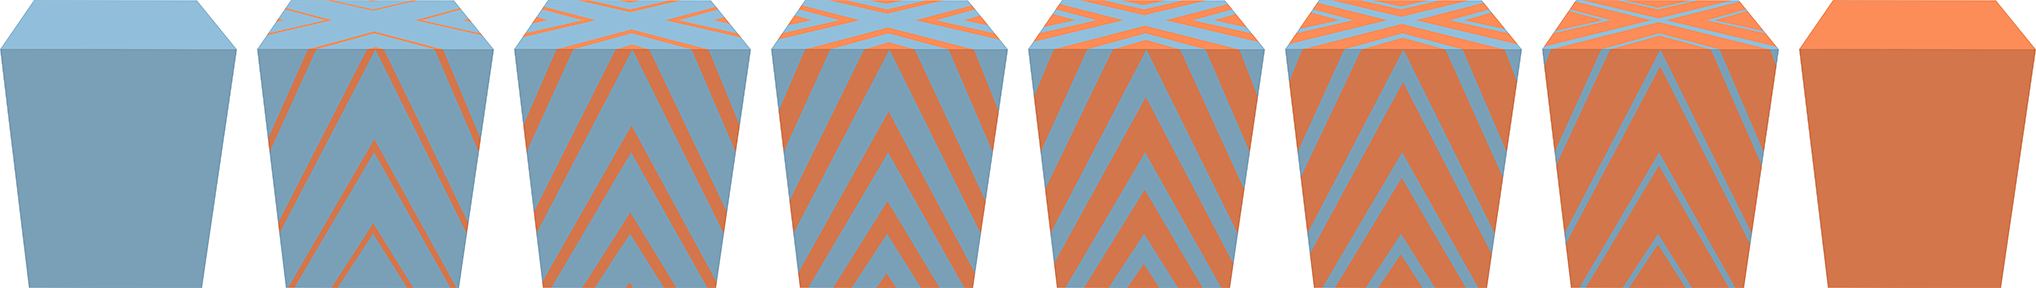
\includegraphics[width=1.0\linewidth]{figures/arrow-trans-vars-variants-full}};%
        \node[below=3.0cm of arrows1.south,anchor=west](arrows2) at (0,0) {%
           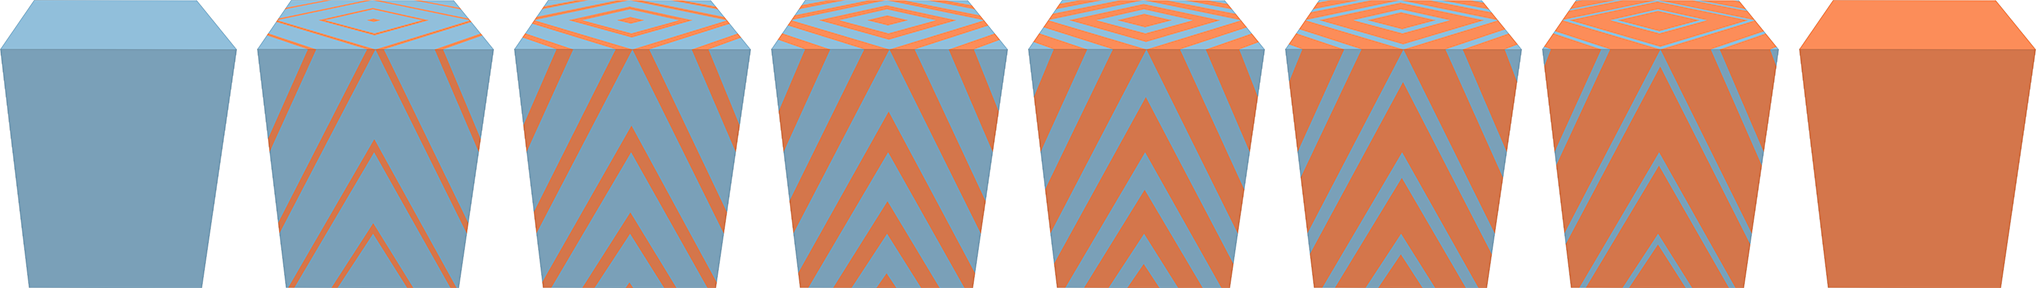
\includegraphics[width=1.0\linewidth]{figures/arrow-trans-vars-variants-full-inverse}};%
        \spy [white] on ($(arrows0.center)+(+0.45, +0.325)$) in node at ($(+2.0, +0.25)+(arrows0.center)$);
        \spy [white] on ($(arrows1.center)+(+0.45, +0.325)$) in node at ($(+2.0, +0.25)+(arrows1.center)$);
        \spy [white] on ($(arrows2.center)+(+0.45, +0.325)$) in node at ($(+2.0, +0.25)+(arrows2.center)$);
    \end{tikzpicture}
    \caption{Temporal variants of the arrow-pattern transition for increasing values: lateral face first, then top face (top), or lateral and top faces simultaneously (center and bottom). 
    }
    \label{fig:arrow-trans-vars-variants}
\end{figure}

\paragraph{Arrows (full)}
This pattern extends the arrow pattern by additional arrows on the top.
Their direction allows for multiple variants (\autoref{fig:arrow-trans-vars-variants}):
For one, they can be appended to the transition of the lateral faces.
This allows an encoding of direction on top only for a short duration of the transition.
Alternatively, the arrows can be animated on the top faces for the whole duration of the transition, whereby two variants with opposite directions are available.

\subsection{Pattern Composition and Contours}
Invariant to all patterns is that not both the direction of animation and the direction of value change can be encoded at the same time.
As further indicator for the direction of animation, we propose a combination of patterns.
Thereby, one of the two distinctly colored areas is superimposed by an additional pattern~(\autoref{fig:trans-vars-combinations}).
This allows for direct unambiguous display of change direction, both when paused and animated, as only one state has a second pattern superimposed.
The shape of the pattern remains unchanged ($t=0.5$) during the transition.
However, as the overall transition changes the surfaces encoding former and next color, the application of the secondary pattern will vary during the transition.
\begin{figure}[t]
    \begin{tikzpicture}[spy using outlines={white, rectangle, magnification=2.5, size=32, connect spies, every spy on node/.append style={line width=1.0pt}},inner sep=0pt, outer sep=0pt]
        \node[anchor=west](arrows0) at (0,0) {%
            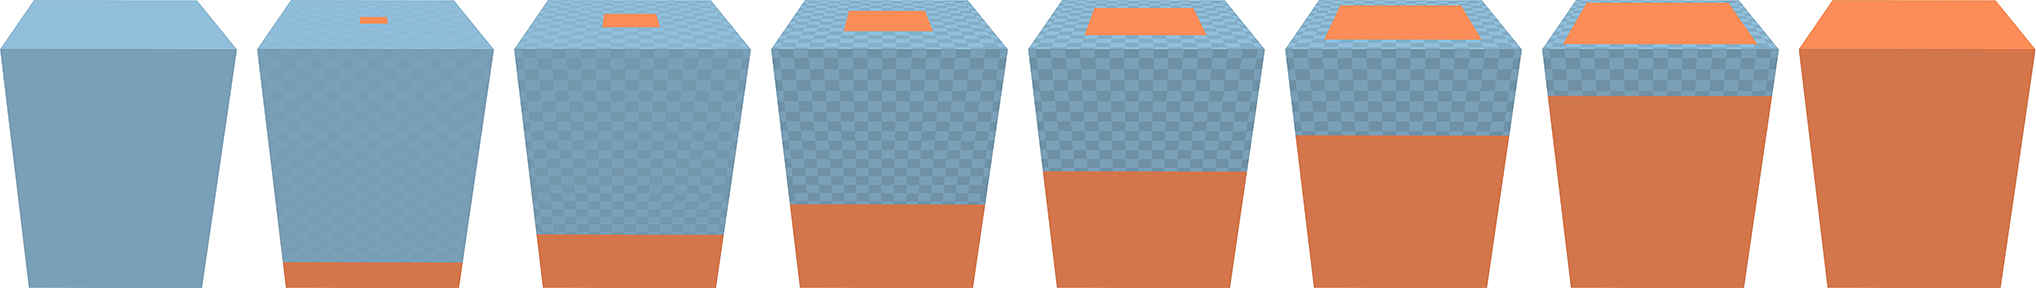
\includegraphics[width=1.0\linewidth]{figures/trans-vars-combinations-pyramid-quads}};
        \node[below=1.5cm of arrows0.south,anchor=west](arrows1) at (0,0) {%
           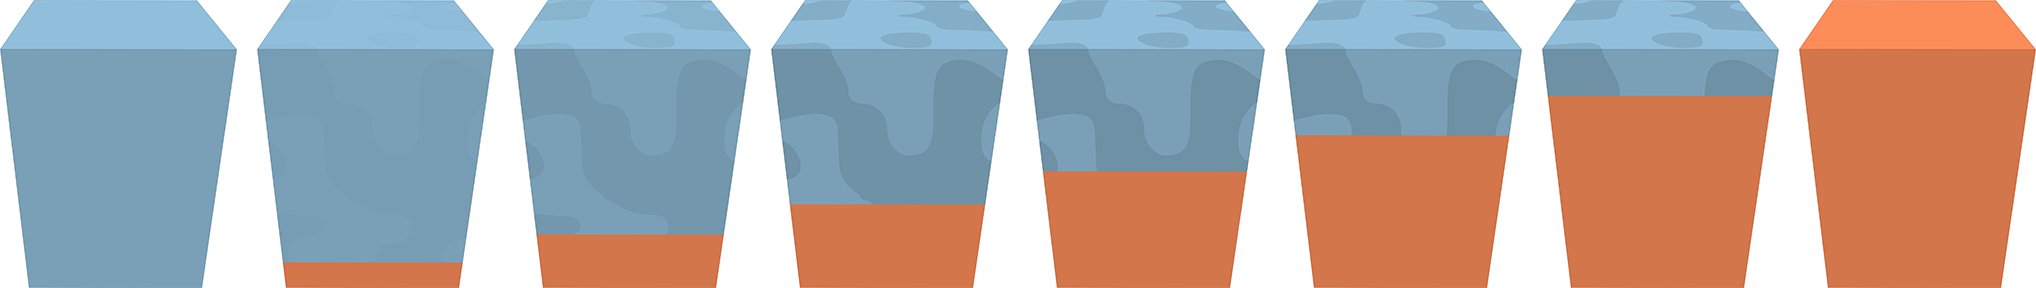
\includegraphics[width=1.0\linewidth]{figures/trans-vars-combinations-vertical-noise}};%
        \node[below=3.0cm of arrows1.south,anchor=west](arrows2) at (0,0) {%
           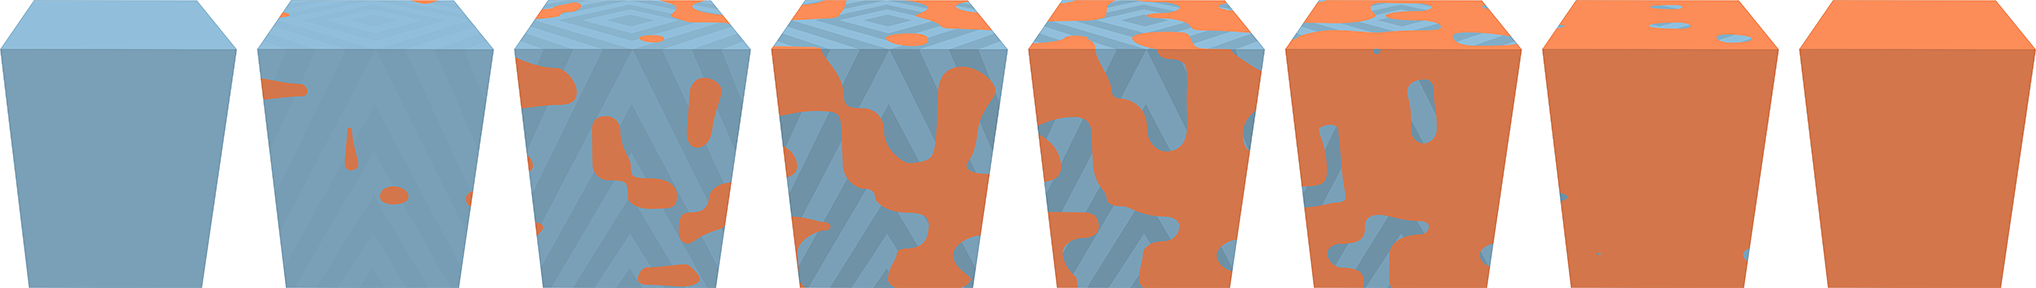
\includegraphics[width=1.0\linewidth]{figures/trans-vars-combinations-noise-arrow-full}};%
        \spy [white] on ($(arrows0.center)+(+0.45, +0.325)$) in node at ($(+2.0, +0.25)+(arrows0.center)$);
        \spy [white] on ($(arrows1.center)+(+0.45, +0.325)$) in node at ($(+2.0, +0.25)+(arrows1.center)$);
        \spy [white] on ($(arrows2.center)+(+0.45, +0.325)$) in node at ($(+2.0, +0.25)+(arrows2.center)$);
    \end{tikzpicture}
    \caption{Combination of two procedural patterns. The dominant pattern is supported by a secondary pattern placed only on the parts representing either the former (as can be seen here) or the upcoming value. }
    \label{fig:trans-vars-combinations}
\end{figure}

\paragraph{Candidates for Secondary Use}
Technically, the secondary pattern is not limited by the choice of the main pattern.
However, we suggest using a different, distinct pattern w.r.t. the main one, ideally one that has a uniform distribution of colors.
Both approaches ensure that the pattern is (1) distinguishable from the main pattern and (2) visible without regard to the current transition state.

\paragraph{Parameterization of Secondary Pattern}
The secondary pattern itself is derived for a static transition value of $t = 0.5$ and applied using blending of the base color and a slightly darker variant.
This way, the pattern occupies half the area of the applied surface.
Regarding the choice of the applied surface, we propose to use the surface that encodes the former color to superimpose the second pattern.
When using the former color, the advantage is that the secondary pattern can be used until the end of the transition, as the surface of former color will vanish during the transition.
In addition, the secondary pattern must not be faded in completely directly at the beginning of the transition.
Otherwise, if an animation consists of several transitions, the secondary pattern would appear abruptly when two transitions are changed.
Therefore, the secondary pattern is faded in gradually with the help of an easing.

\subsection{Transitions and Animations}
So far, we considered isolated transitions from one color to another for a single node.
In order to display multiple changes over multiple snapshots of data, we consider the use of animations.

\paragraph{Transition}
A transition describes a change from a node's state or mapped value to another one.
Thereby, a transition will not encode time or duration but only progress.
The required parameter for such a transition is its progress control $t \in [0, 1]$ where $0$ is used at the start and $1$ at the end of a transition.

\paragraph{Animation}
Animation is the continuous progression over multiple states by means of transitions.
More importantly, it is linked to the concept of time and duration.
Note that the transitions can be enhanced by easing functions which is not discussed in this context~\cite{Thomas81}.
The animation between two points in time, e.g., two subsequent revisions for software system data, can range from running all transitions for every node and every visual variable in parallel as well as in strict sequence.
The former approach is strictly limited by the number of concurrent changes (\autoref{fig:oh-my-clutter}).
\begin{figure}[t]
    \begin{tikzpicture}[spy using outlines={black, rectangle, magnification=4.0, size=76, connect spies, every spy on node/.append style={line width=1.0pt}},inner sep=0pt, outer sep=0pt]
        \node[anchor=west](arrows0) at (0.0,0) {%
            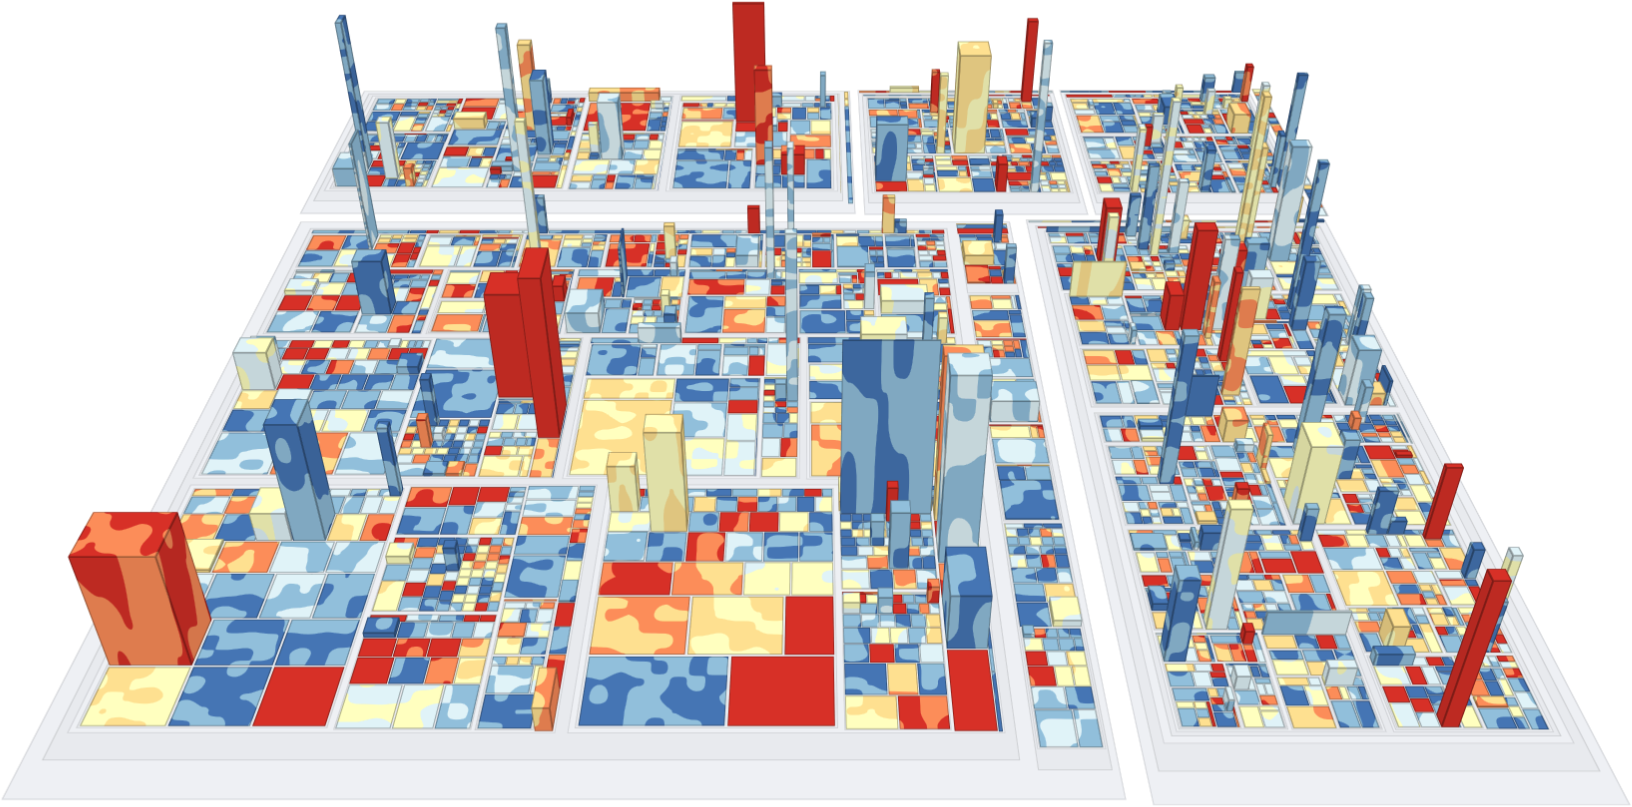
\includegraphics[width=0.6666\linewidth, trim=0 16 0 16, clip]{figures/all-transitions-at-once}};
        \spy [white] on ($(arrows0.center)+(+1.5, -0.5)$) in node at ($(+4.2, +0.0)+(arrows0.center)$);
    \end{tikzpicture}
    \caption{Example of an extreme case with all color transitions of all nodes being shown at once with $t=0.5$.}
    \label{fig:oh-my-clutter}
\end{figure}

\section{Discussion}
\label{sec:evaluation}
Our prototype extends an existing, WebGL-based rendering system for large-scale 2D and 2.5D treemaps.
The implementation of the patterns itself was straightforward and imposed no significant impact on rendering performance (runs on mobile devices for large treemaps).
For the animation in general, we had to redesign large parts of our visualization and rendering implementation though.
In the remainder of this section we briefly discuss some animation aspects and assess the applicability of our patterns.

\subsection{Animation Controller}
We composed the handling of animations and transitions into a system that manages all temporal animations, controlling the time-dependent transition values as well as the individual, per-node transition states (\autoref{fig:teaser}).
Thereby, our prototype allows for independent, simultaneous transitions per-node, for every mapped data attribute.
The procedural patterns are implemented as temporal visual variables, mapping a 3-tuple (a value per state and transition progress) to color instead of a single value.
An animation of weight and height mappings is implemented similarly.
The latter allows for ordering and masking of transitions based on (1) transition type, (2) arbitrary node associated values, (3) meta data, or (4) enumeration and more.
With this starting point, we have begun to identify meaningful applications within this design space.
\begin{figure}[b]
    \begin{tikzpicture}[spy using outlines={white, rectangle, magnification=2.5, size=32, connect spies, every spy on node/.append style={line width=1.0pt}},inner sep=0pt, outer sep=0pt]
        \node[anchor=west](arrows0) at (0,0) {%
            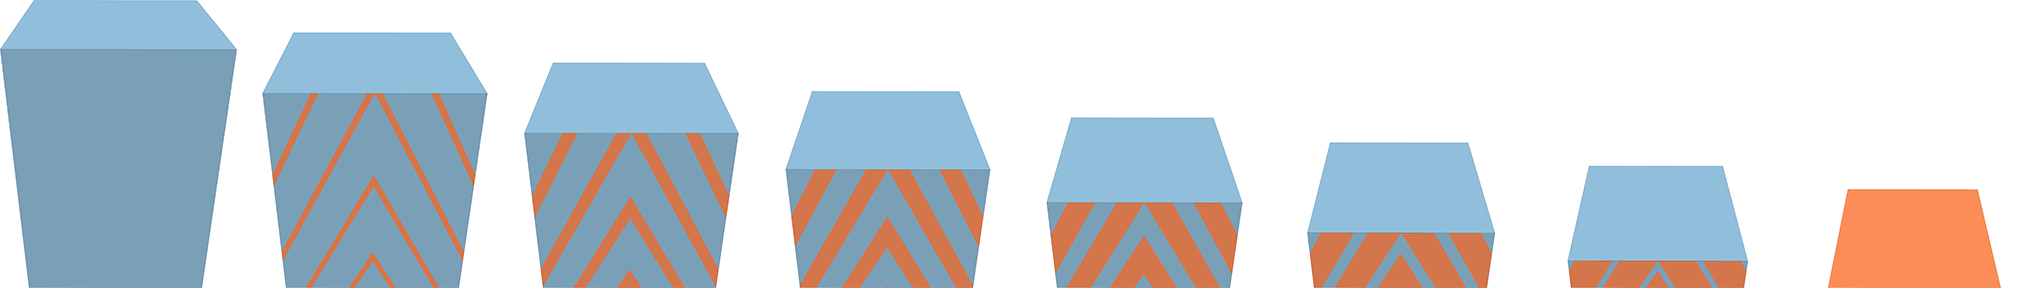
\includegraphics[width=1.0\linewidth]{figures/color-and-height-change-arrows}};
        \node[below=1.5cm of arrows0.south,anchor=west](arrows1) at (0,0) {%
           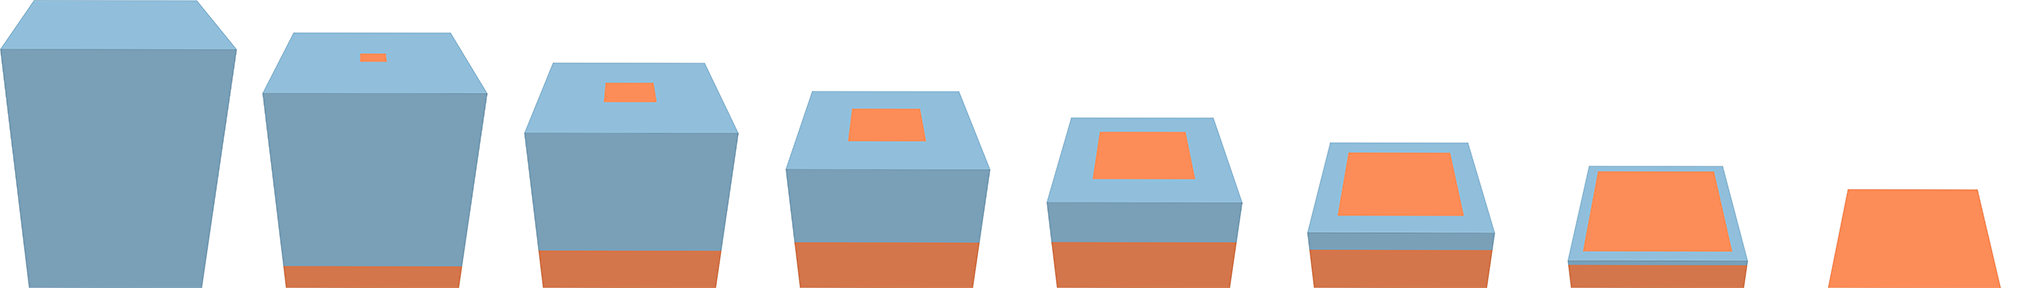
\includegraphics[width=1.0\linewidth]{figures/color-and-height-change-pyramid}};%
    \end{tikzpicture}
    \caption{Example of two patterns used for a transition of simultaneous increase in color and decrease in height values.}
    \label{fig:color-and-height-change}
\end{figure}

\subsection{Qualitative Assessment}
\begin{table}[t]
    \centering
    \renewcommand{\arraystretch}{1.3}
    \rowcolors{3}{white}{gray!10}%
    \setlength{\tabcolsep}{5pt}%
    \caption{Overview of the patterns and their characteristics.\\
    Notation: \OK~supported | \PARTIAL~partial support | --~unsupported.\vspace{-0.75\baselineskip}} %
    \begin{tabularx}{\linewidth}{rXccccccc}
        \multicolumn{2}{l}{\textbf{Procedural Pattern}} &
        \rot{\makecell[l]{\strut $\Delta_{\textrm{DirAnim}}$}}   &
        \rot{\makecell[l]{\strut $\Delta_{\textrm{DirChange}}$}} &
        \rot{\makecell[l]{\strut $\Delta_{\textrm{RatioLat}}$}}  &
        \rot{\makecell[l]{\strut $\Delta_{\textrm{RatioTop}}$}}  &
        \rot{\makecell[l]{\strut $\Delta_{\textrm{IndHeight}}$}} &
        \rot{\makecell[l]{\strut $\Delta_{\textrm{IndWeight}}$}} &
        \rot{\makecell[l]{\strut $\Delta_{\textrm{TreeSize}}$}}  \\
        \hline
        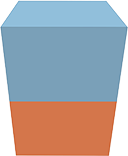
\includegraphics[height=1.4em]{figures/vertical-50-dark-sm-alpha}    & \strut \small%
            Pillar         & \OK & -- & \PARTIAL & --  & --  & \OK      & \OK \\
        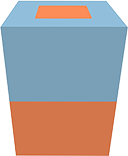
\includegraphics[height=1.4em]{figures/pyramid-50-dark-sm-alpha}     & \strut \small%
            Pyramid        & \OK & -- & \OK      & \OK & --  & \PARTIAL & \OK \\
        
\includegraphics[height=1.4em]{figures/dithering-50-dark-sm-alpha}   & \strut \small%
            Dithering      & --  & -- & \OK      & \OK & \OK & \OK      & \OK \\
        
\includegraphics[height=1.4em]{figures/arrows-50-dark-sm-alpha}      & \strut \small%
            Arrows         & -- & \OK & \PARTIAL & --  & \OK & \OK      & \OK \\
        
\includegraphics[height=1.4em]{figures/arrows-full-50-dark-sm-alpha} & \strut \small%
            Arrows (full)  & -- & \OK & \OK      & \OK & \OK & \OK      & \OK \\
        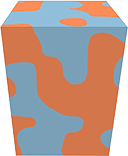
\includegraphics[height=1.4em]{figures/noise-50-dark-sm-alpha}       & \strut \small%
            Noise          & --  & -- & --       & \OK & \OK & \OK      & --  \\
        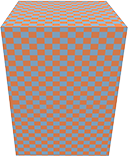
\includegraphics[height=1.4em]{figures/quads-50-dark-sm-alpha}       & \strut \small%
            Squares        & --  & -- & \OK      & \OK & \OK & \OK      & --  \\
    \end{tabularx}
    \label{tab:template-characteristics}
\end{table}
We assessed the temporal visual variables, using every pattern individually and in combination, and applied them for weight, height, and color change emphasis on small and large real-world data sets.
For the scope of this work, we derive the following characteristics:
\newlength{\maxlabel}
\setlength{\maxlabel}{\widthof{$\Delta_{\textrm{DirChange}}$}+1em}
\begin{description}[itemindent=0mm,labelwidth=20mm,leftmargin=\maxlabel,align=right,itemsep=1mm]
    \item [$\Delta_{\textrm{DirAnim}}$]
        The direction of animation can be read unambiguously while the animation is paused in a transition.
    \item [$\Delta_{\textrm{DirChange}}$]
        The direction of change in value can be read unambiguously while the animation is paused.
    \item [$\Delta_{\textrm{RatioLat}}$]
        The ratio of different colors on the lateral faces matches a transition's progress.
    \item [$\Delta_{\textrm{RatioTop}}$]
        The ratio of different colors on the top face matches a transition's progress (top view or 2D treemap).
    \item [$\Delta_{\textrm{IndHeight}}$]
        The mapping of change difference and change direction does not compromise the height mapping.
    \item [$\Delta_{\textrm{IndWeight}}$]
        The mapping of change difference and change direction does not compromise the weight mapping.
    \item [$\Delta_{\textrm{TreeSize}}$]
        The pattern can be easily adjusted for large or very large treemaps.
\end{description}
We assessed all proposed patterns on real data sets by their degree to satisfy the characteristics (\autoref{tab:template-characteristics}).
We conclude that no pattern satisfies all desired characteristics.
However, we want to highlight the arrows (full) pattern that supports most of the characteristics.

\section{Conclusions} 
The proposed system supports display of changes in all of treemap item areas, heights using geometry displacement, and colors using animated procedural textures.
This is relevant for the exploration of time-varying data such as software data.
As a special requirement we introduced the readability for both a static image and a dynamic animated transition.
For specific templates on how to transition color values in 3D we proposed the seven variants (1) \emph{pillar}, (2) \emph{pyramid}, (3) \emph{arrows}, (4) \emph{arrows (full)}, (5) \emph{noise}, (6) \emph{dithering}, and (7) \emph{squares}.
We discussed the different characteristics, especially direction of change and direction of animation, strengths, and weaknesses of each template but cannot draw a conclusion on a default template at this point.
However, we found that using the time control helps to understand the changes of individual nodes.

For future work, we plan to perform quantitative evaluations by means of comprehensive user studies and extended case studies on large software systems and long time spans.

\begin{acks}
    This work has been supported by the German Federal Ministry of Education and Research (BMBF) through grant 01IS19006  (\enquote{KI-Labor ITSE}).
    Further, this work is part of the \enquote{Software-DNA} project, which is funded by the European Regional Development Fund (ERDF or EFRE in German) and the State of Brandenburg (ILB), and the \enquote{TASAM} project, which is funded by the German Federal Ministry for Economic Affairs and Energy (BMWi, ZIM).
\end{acks}

\bibliographystyle{ACM-Reference-Format}
\bibliography{references}

\end{document}
\endinput
